\documentclass[tikz,border=8mm]{standalone}
\usepackage[T1]{fontenc}
\usepackage[utf8]{inputenc}
\usepackage{lmodern}
\usepackage{amsmath}
\usepackage{xcolor}
\usetikzlibrary{arrows.meta,calc,positioning}

\definecolor{ArrowBlue}{HTML}{1877F2}
\definecolor{DeepBlue}{HTML}{104A89}
\definecolor{QHeader}{HTML}{BFE6C3}
\definecolor{KHeader}{HTML}{BCD9F6}
\definecolor{Q0Fill}{HTML}{FFA9A9}
\definecolor{Q1Fill}{HTML}{FFC06B}
\definecolor{Q2Fill}{HTML}{F3EE74}
\definecolor{QDotsFill}{HTML}{98EB8D}
\definecolor{QiFill}{HTML}{9ECAF7}
\definecolor{KFill}{HTML}{CFE3F7}
\definecolor{GreenAccent}{HTML}{1F7A3F}
\definecolor{FrameGray}{HTML}{D3DCE8}
\definecolor{InfoFill}{HTML}{EEF3F9}

\begin{document}
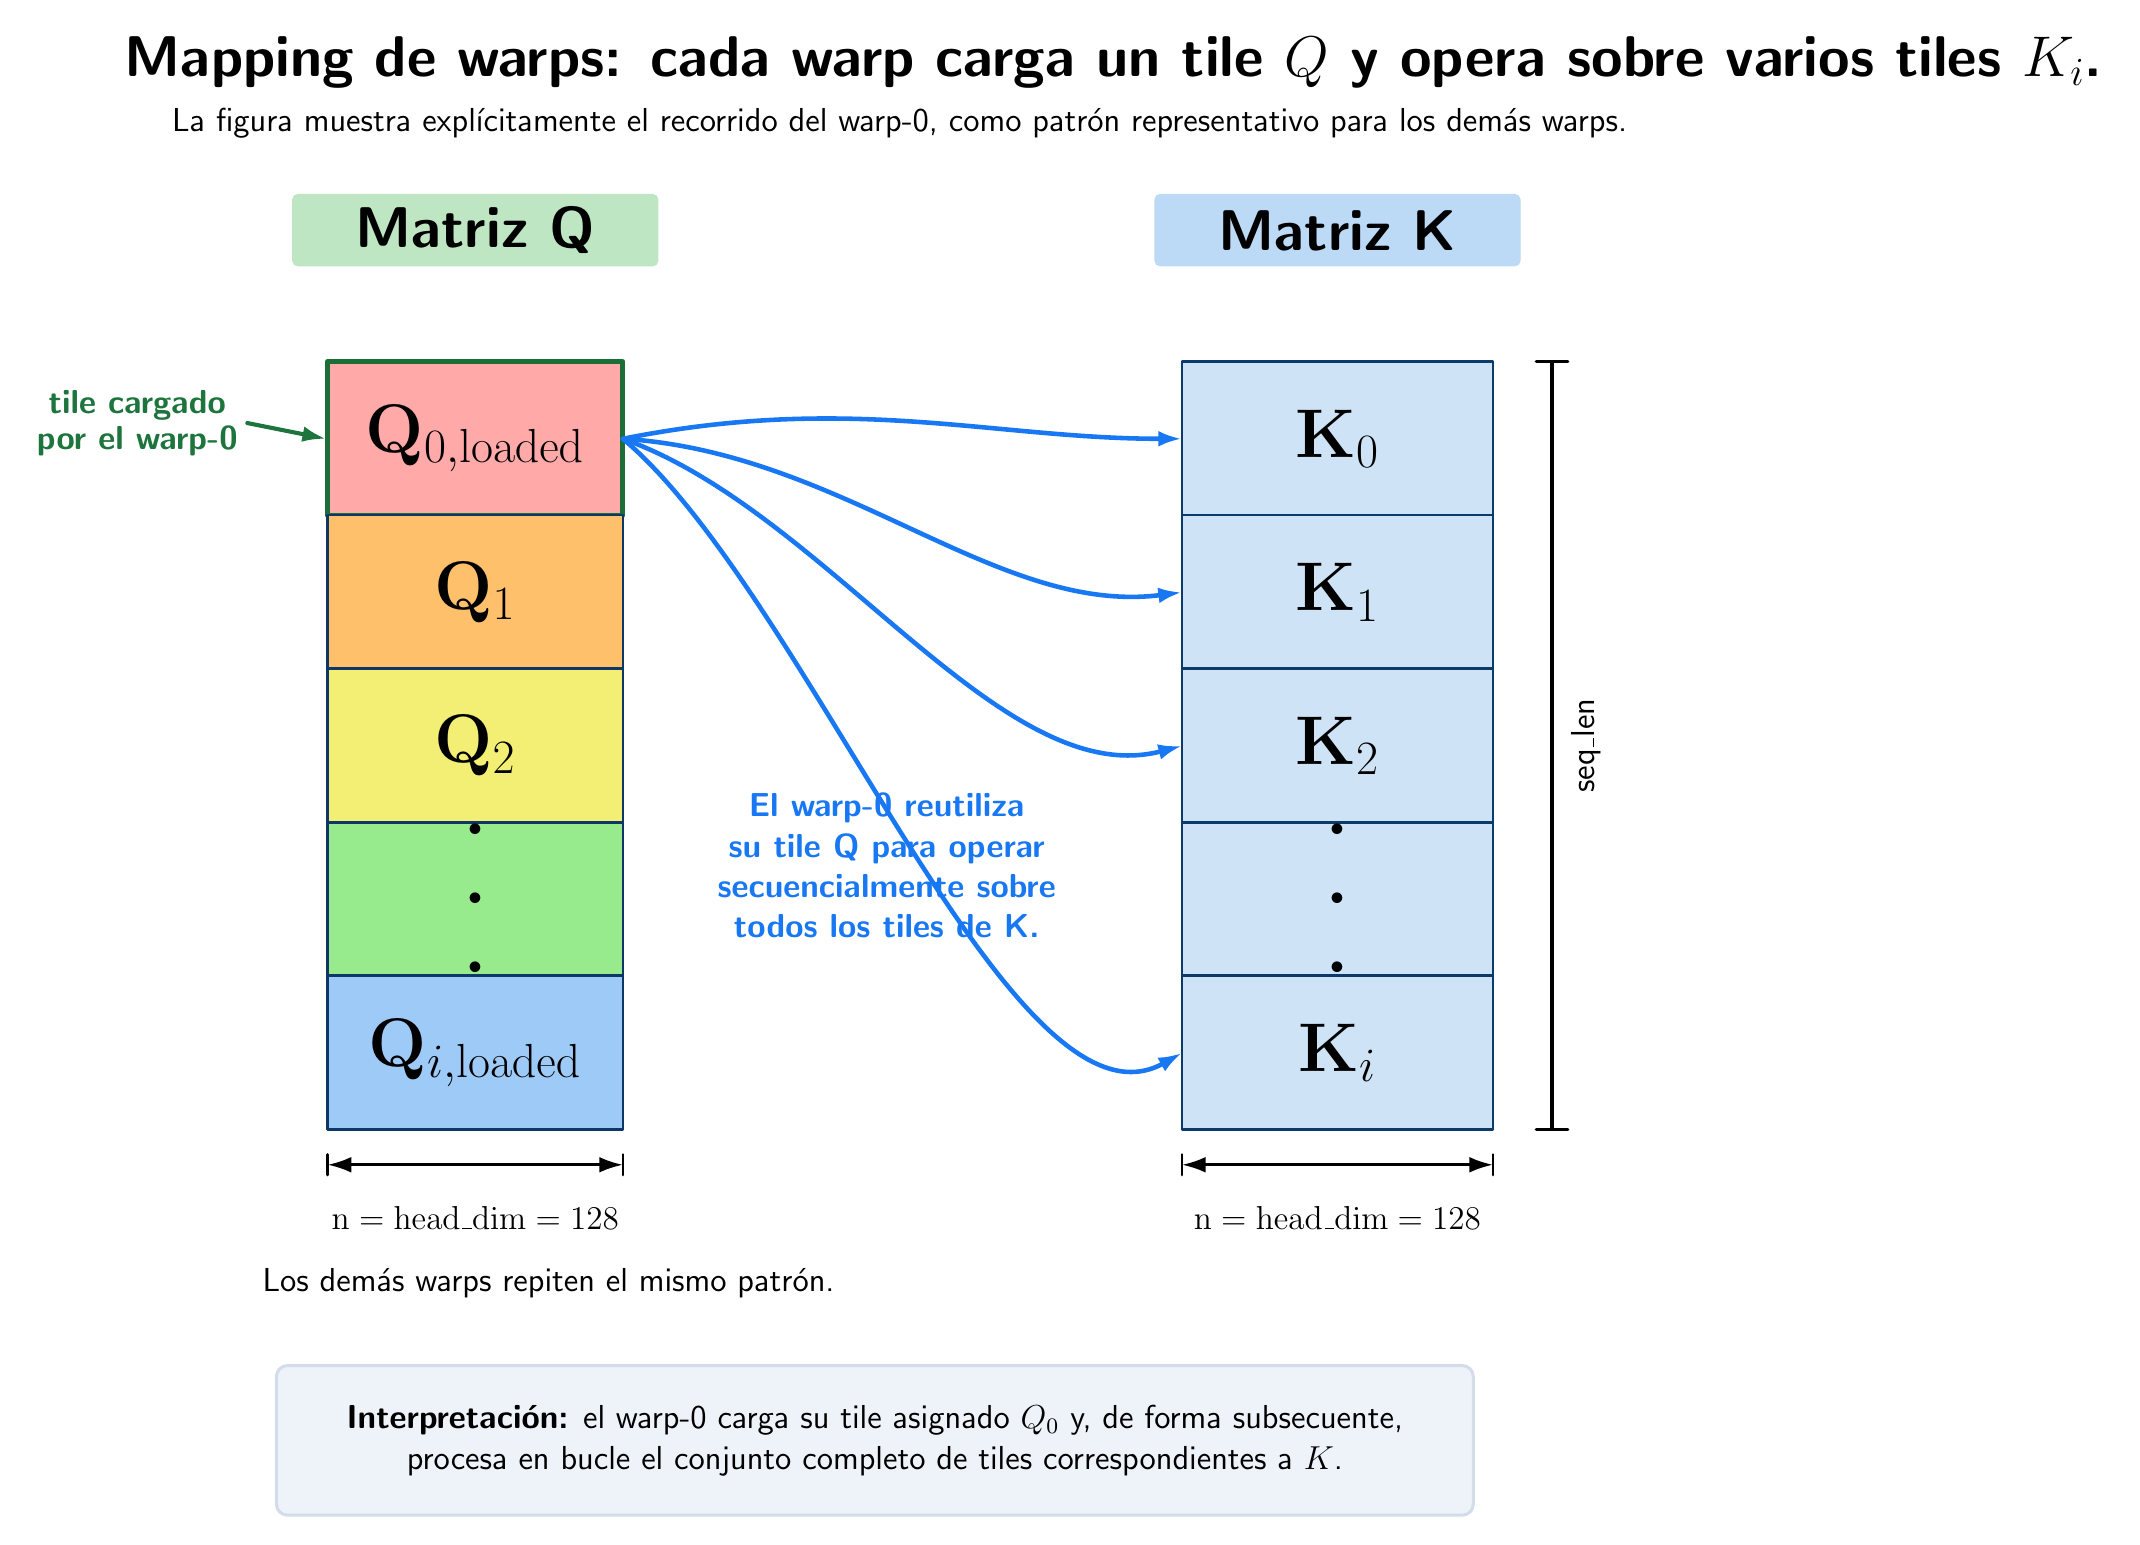
\begin{tikzpicture}[x=1cm,y=1cm, line cap=round, line join=round, >={Latex[length=3mm,width=2mm]}]

% title
\node[anchor=west,font=\sffamily\bfseries\fontsize{22}{24}\selectfont,text=black] at (-2.7,2.55)
{Mapping de warps: cada warp carga un tile $Q$ y opera sobre varios tiles $K_i$.};
\node[anchor=west,font=\sffamily\fontsize{12.5}{15}\selectfont,text=black] at (-2.1,1.78)
{La figura muestra explícitamente el recorrido del warp-0, como patrón representativo para los demás warps.};

% headers
\node[rounded corners=2pt, fill=QHeader, minimum width=4.65cm, minimum height=0.92cm,
      font=\sffamily\bfseries\fontsize{20}{22}\selectfont] at (1.875,0.42) {Matriz Q};
\node[rounded corners=2pt, fill=KHeader, minimum width=4.65cm, minimum height=0.92cm,
      font=\sffamily\bfseries\fontsize{20}{22}\selectfont] at (12.825,0.42) {Matriz K};

% Q blocks coordinates: x from 0 to 3.75, heights 1.95
% Q0
\fill[Q0Fill] (0,-1.25) rectangle (3.75,-3.20);
\draw[GreenAccent!90!black,line width=1.8pt] (0,-1.25) rectangle (3.75,-3.20);
\node[font=\sffamily\bfseries\fontsize{23}{25}\selectfont] at (1.875,-2.23) {$\mathbf{Q}_{0,\mathrm{loaded}}$};
% Q1
\fill[Q1Fill] (0,-3.20) rectangle (3.75,-5.15);
\draw[DeepBlue!75!black,line width=0.95pt] (0,-3.20) rectangle (3.75,-5.15);
\node[font=\sffamily\bfseries\fontsize{23}{25}\selectfont] at (1.875,-4.18) {$\mathbf{Q}_{1}$};
% Q2
\fill[Q2Fill] (0,-5.15) rectangle (3.75,-7.10);
\draw[DeepBlue!75!black,line width=0.95pt] (0,-5.15) rectangle (3.75,-7.10);
\node[font=\sffamily\bfseries\fontsize{23}{25}\selectfont] at (1.875,-6.13) {$\mathbf{Q}_{2}$};
% Qdots
\fill[QDotsFill] (0,-7.10) rectangle (3.75,-9.05);
\draw[DeepBlue!75!black,line width=0.95pt] (0,-7.10) rectangle (3.75,-9.05);
\node[font=\sffamily\bfseries\fontsize{24}{26}\selectfont,align=center] at (1.875,-8.08) {$\boldsymbol{\cdot}$\\[-1pt]$\boldsymbol{\cdot}$\\[-1pt]$\boldsymbol{\cdot}$};
% Qi
\fill[QiFill] (0,-9.05) rectangle (3.75,-11.00);
\draw[DeepBlue!75!black,line width=0.95pt] (0,-9.05) rectangle (3.75,-11.00);
\node[font=\sffamily\bfseries\fontsize{23}{25}\selectfont] at (1.875,-10.03) {$\mathbf{Q}_{i,\mathrm{loaded}}$};

% left label arrow
\node[anchor=east, align=center, font=\sffamily\bfseries\fontsize{11.5}{13.2}\selectfont, text=GreenAccent!95!black] (loadedtxt) at (-1.02,-2.03)
{tile cargado\\por el warp-0};
\draw[->, GreenAccent!95!black, line width=1.5pt] (loadedtxt.east) -- (-0.02,-2.23);

% K blocks x from 10.85 to 14.80, same height with gaps
% K0
\fill[KFill] (10.85,-1.25) rectangle (14.80,-3.20);
\draw[DeepBlue!78!black,line width=0.95pt] (10.85,-1.25) rectangle (14.80,-3.20);
\node[font=\sffamily\bfseries\fontsize{24}{26}\selectfont] at (12.825,-2.23) {$\mathbf{K}_{0}$};
% K1
\fill[KFill] (10.85,-3.20) rectangle (14.80,-5.15);
\draw[DeepBlue!78!black,line width=0.95pt] (10.85,-3.20) rectangle (14.80,-5.15);
\node[font=\sffamily\bfseries\fontsize{24}{26}\selectfont] at (12.825,-4.18) {$\mathbf{K}_{1}$};
% K2
\fill[KFill] (10.85,-5.15) rectangle (14.80,-7.10);
\draw[DeepBlue!78!black,line width=0.95pt] (10.85,-5.15) rectangle (14.80,-7.10);
\node[font=\sffamily\bfseries\fontsize{24}{26}\selectfont] at (12.825,-6.13) {$\mathbf{K}_{2}$};
% Kdots
\fill[KFill] (10.85,-7.10) rectangle (14.80,-9.05);
\draw[DeepBlue!78!black,line width=0.95pt] (10.85,-7.10) rectangle (14.80,-9.05);
\node[font=\sffamily\bfseries\fontsize{24}{26}\selectfont,align=center] at (12.825,-8.08) {$\boldsymbol{\cdot}$\\[-1pt]$\boldsymbol{\cdot}$\\[-1pt]$\boldsymbol{\cdot}$};
% Ki
\fill[KFill] (10.85,-9.05) rectangle (14.80,-11.00);
\draw[DeepBlue!78!black,line width=0.95pt] (10.85,-9.05) rectangle (14.80,-11.00);
\node[font=\sffamily\bfseries\fontsize{24}{26}\selectfont] at (12.825,-10.03) {$\mathbf{K}_{i}$};

% arrows from Q0_loaded to K tiles
\coordinate (Q0out) at (3.75,-2.23);
\draw[->, ArrowBlue, line width=1.65pt] (Q0out) .. controls (6.65,-1.65) and (8.45,-2.23) .. (10.85,-2.23);
\draw[->, ArrowBlue, line width=1.65pt] (Q0out) .. controls (6.55,-2.40) and (8.50,-4.48) .. (10.85,-4.18);
\draw[->, ArrowBlue, line width=1.65pt] (Q0out) .. controls (6.35,-3.15) and (8.55,-6.73) .. (10.85,-6.13);
\draw[->, ArrowBlue, line width=1.65pt] (Q0out) .. controls (6.10,-4.20) and (8.70,-11.23) .. (10.85,-10.03);

% central explanation
\node[align=center, font=\sffamily\bfseries\fontsize{12.5}{14.5}\selectfont, text=ArrowBlue] at (7.10,-7.65)
{El warp-0 reutiliza\\su tile Q para operar\\secuencialmente sobre\\todos los tiles de K.};

% bottom-left note
\node[anchor=west, font=\sffamily\fontsize{12.5}{14}\selectfont] at (-0.95,-12.95)
{Los demás warps repiten el mismo patrón.};

% dimensions
\draw[<->, black, line width=1.0pt] (0,-11.45) -- (3.75,-11.45);
\draw[black, line width=1.0pt] (0,-11.32) -- (0,-11.58);
\draw[black, line width=1.0pt] (3.75,-11.32) -- (3.75,-11.58);
\node[font=\sffamily\fontsize{12.5}{14}\selectfont,align=center] at (1.875,-12.12)
{$\mathrm{n}=\mathrm{head\_dim}=128$};

\draw[<->, black, line width=1.0pt] (10.85,-11.45) -- (14.80,-11.45);
\draw[black, line width=1.0pt] (10.85,-11.32) -- (10.85,-11.58);
\draw[black, line width=1.0pt] (14.80,-11.32) -- (14.80,-11.58);
\node[font=\sffamily\fontsize{12.5}{14}\selectfont,align=center] at (12.825,-12.12)
{$\mathrm{n}=\mathrm{head\_dim}=128$};

\draw[black, line width=1.2pt] (15.55,-1.25) -- (15.55,-11.00);
\draw[black, line width=1.2pt] (15.35,-1.25) -- (15.75,-1.25);
\draw[black, line width=1.2pt] (15.35,-11.00) -- (15.75,-11.00);
\node[rotate=90,font=\sffamily\fontsize{13}{15}\selectfont] at (15.98,-6.13) {seq\_len};

% interpretation box
\node[rounded corners=4pt, draw=FrameGray, fill=InfoFill, line width=1.1pt,
      minimum width=15.2cm, minimum height=1.90cm, align=center, inner sep=9pt,
      font=\sffamily\fontsize{11.8}{14.8}\selectfont, text=black] at (6.95,-14.95)
{\textbf{Interpretación:} el warp-0 carga su tile asignado $Q_0$ y, de forma subsecuente,\\
 procesa en bucle el conjunto completo de tiles correspondientes a $K$.};

\end{tikzpicture}
\end{document}
